\section{Introduction}
\label{sec:introduction}

When language models train iteratively on their own output, the training distribution progressively loses its tail modes, a phenomenon termed model collapse~\citep{shumailov2024curse,alemohammad2024mad}.
This process can be triggered by vanishingly small synthetic fractions~\citep{dohmatob2025strong}: lexical diversity narrows, calibration deteriorates, and each generation inherits the biases of its predecessors.
As machine-generated text grows prevalent on the web, such feedback loops pose a growing risk to production pipelines, and by the time standard quality metrics register degradation, the distribution may have already shifted irreversibly.

This threat motivates a fundamental question: \emph{can we reliably detect the onset of model collapse?}
The answer is less clear than it might appear.
Iterative training produces short, noisy time series (often fewer than 15 points) where detection power drops sharply~\citep{boettiger2012limits}, and model collapse is a first-order transition~\citep{truong2026phase}, structurally ruling out the critical-slowing-down early-warning signals that ecologists rely on~\citep{scheffer2009early} (\S\ref{sec:related_work}).
More fundamentally, no prior work has systematically compared detection methods on this problem; as we show, the choice of statistical test alone can shift conclusions from universal detection to complete null on identical data.

We systematically map this \emph{detectability landscape}---how detection outcomes vary across contamination levels ($\alpha$), observation windows ($T$), and statistical methods---on Pythia-410M~\citep{biderman2023pythia} across 13 contamination levels with multi-seed replication (Figure~\ref{fig:phase_diagram}).
Our central finding is a sharp detection phase transition: Permutation Granger causality (PermG) finds 0/8 significant canary$\to$downstream pairs through $\alpha{=}0.45$, then jumps to 6/8 within a 2-percentage-point interval at $\alpha{=}0.50$ (Figure~\ref{fig:phase_diagram}), defining an empirical detection boundary $\alpha_c(T)$ (Eq.~\ref{eq:alpha-c}) that organizes three confirmed regimes (blind, onset, detection) plus one non-monotonic anomaly.
This transition emerges from a five-method comparison that itself reveals dramatic method sensitivity: null-control FPR spans 6.7\% to 94.4\% ($\kappa{=}0.185$; Figure~\ref{fig:method_comparison}), demonstrating that single-method analyses cannot reliably distinguish real signals from artifacts.
Cross-architecture evaluation at $\alpha{=}1.0$ across five families (345M--6.9B) supports forward detection in 11/15 conditions, with four non-confirming cases isolating distinct failure modes (\S\ref{sec:generalization}).
Our canary claim is scoped to diversity metrics (distinct-$n$~\citep{li2016diversity}); Granger precedence establishes temporal predictive improvement, not causation (\S\ref{sec:method}).

Our contributions are:\footnote{Code and data: \url{https://github.com/anonymous-nlp-2026-2/distrib_canary_collapse}}
\begin{enumerate}
    \item \textbf{We identify a sharp detection phase transition} (\S\ref{sec:regime}--\ref{sec:dose_response}).
    Detection jumps from 0/8 to 6/8 significant pairs within 2 percentage points of $\alpha_c \approx 0.50$, defining three confirmed regimes (blind, onset, detection) plus a non-monotonic anomaly at $\alpha \approx 0.60$.

    \item \textbf{We map the detectability landscape} across contamination levels and observation windows (\S\ref{sec:t20}--\ref{sec:theory}).
    The detection boundary shifts leftward with longer observation, organizing the signal$\times$resolution tradeoff that governs detection feasibility.

    \item \textbf{A multi-method diagnostic toolkit enables these discoveries} (\S\ref{sec:mmct}).
    Five methods yield null-control FPR from 6.7\% to 94.4\% ($\kappa{=}0.185$); systematic comparison identifies PermG (6.7\%, CI $[1.8\%, 16.2\%]$, 10~seeds) as the primary detector and exposes method sensitivity as a key obstacle.

    \item \textbf{We validate practical applications}: a cascade ordering where entropy precedes diversity by ${\geq}1$ generation (Principles~\ref{thm:entropy_leads}--\ref{prop:div_lag}; 14/15 experiments) enables proof-of-concept predictive intervention reducing peak perplexity by 64\% (\S\ref{sec:cascade}, \S\ref{sec:intervention}).
\end{enumerate}

\begin{figure}[t]
\centering
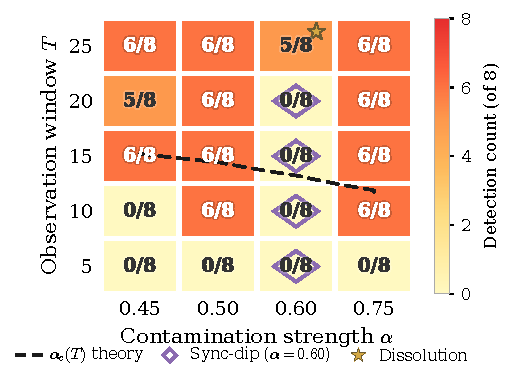
\includegraphics[width=\columnwidth]{figures/fig_phase_diagram.pdf}
\caption{Phase diagram (Pythia-410M, fp32, PermG). FDR-significant canary$\to$diversity pairs across $\alpha$ and $T$; dashed curve: fitted boundary (Eq.~\ref{eq:alpha-c}); $\diamond$: non-monotonic anomaly; $\star$: dissolution at $T{=}25$.}
\label{fig:phase_diagram}
\end{figure}
